\begin{minipage}[t][\PosterFourHeight][t]{\PosterGridWidth}\vspace{0pt}
  \begin{PosterPanel}{\PosterFourHeight}{4}{HOW: A FORMULA FOR THE GAINS AND A REPAIR RULE}

    \noindent\begin{minipage}[t]{268mm}\vspace{0pt}
      {\Subhead\color{IASDarkGreen}A. Gains from a formula, not a search\par}\vspace{1mm}
      {\FigureSize Choose the pole $\lambda$ and a pattern $q$. The PI term must satisfy $(K_p\lambda+K_i)\,y_i=\lambda^{2}(1+t_f\lambda)\,e^{\lambda\tau_i}q_i$. With $W_i$ the right side over $y_i$:\par}
      {\HeroEquation\color{IASBlue}\[
        \begin{gathered}
          K_{p,i}=\dfrac{\Im W_i}{\Im\lambda}\\[1mm]
          K_{i,i}=\Re W_i-\Re\lambda\,K_{p,i}
        \end{gathered}
      \]}
      \vspace{2mm}
      {\FigureSize $y=G(\lambda,\rho)q$: how the grid returns each site's phase error. Needs invertible hidden blocks and gains inside the bounds.\par}
    \end{minipage}\hfill%
    \begin{minipage}[t]{300mm}\vspace{0pt}
      {\Subhead\color{IASDarkGreen}B. Repair rule when retunes interact\par}\vspace{1mm}
      {\FigureSize \StepBadge{1}\ Retune each site alone so the mode keeps its decay.\par}\vspace{1mm}
      {\FigureSize \StepBadge{2}\ Evaluate the joint pole on the full delayed model: this gives $\mathcal I$.\par}\vspace{1mm}
      {\FigureSize \StepBadge{3}\ Give each site $t/2$ extra decay and repeat:\par}
      {\EquationSize\color{IASBlue}\[
        t_{k+1}=\max\{0,\ \mathcal I(t_k)-b\},\quad b=-\alpha_{\text{anchor}}-\sigma
      \]}
      \vspace{-4mm}
      {\FigureSize If $\sup|\mathcal I'|\le L<1$ the update contracts: $|t_k-t^{\star}|\le L^{k}|t_0-t^{\star}|$.\par}
    \end{minipage}\hfill%
    \begin{minipage}[t]{262mm}\vspace{0pt}
      {\Subhead\color{IASDarkGreen}Result of the rule\par}\vspace{1mm}
      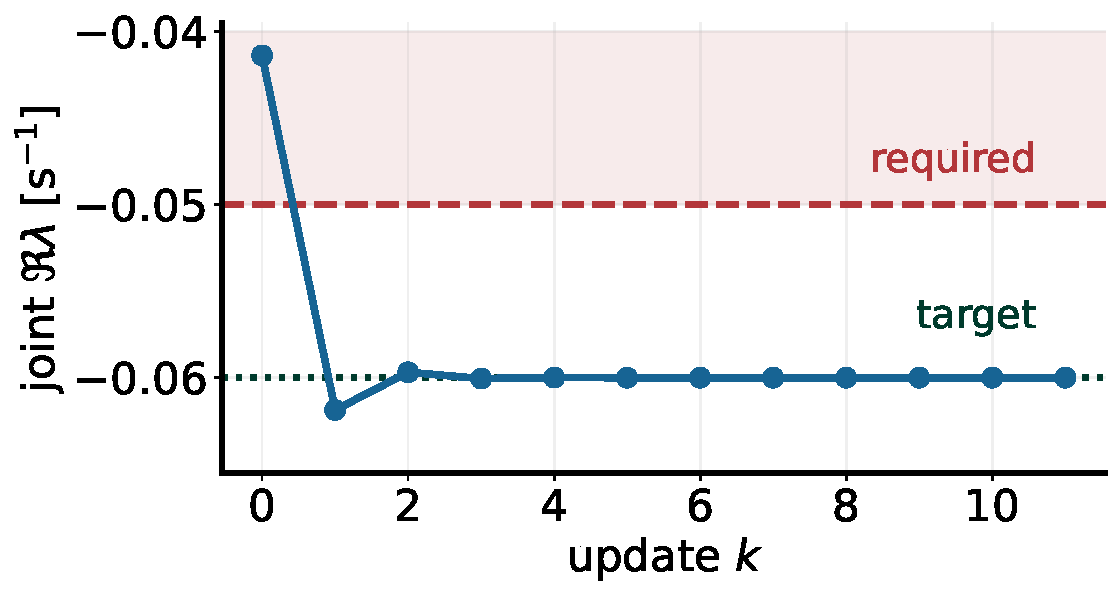
\includegraphics[width=258mm,height=76mm,keepaspectratio]{generated/figures/repair.pdf}\par
      {\FigureSize \textbf{11 updates}: $-0.0414\to-0.0600$. Only $K_i$ moves ($272.42$ and $288.70$); $K_p$ fixed. Sampled slope $\le0.385$.\par}
    \end{minipage}\par
    \vspace{1mm}
    \begin{InWords}\InWordsLabel Choose the pole you want and the gains follow. If two retunes interact, add decay until the interaction no longer eats the margin.\end{InWords}

  \end{PosterPanel}
\end{minipage}%
